\documentclass{ctexart}
\usepackage{tikz, amsmath, pdfpages, placeins, listings}
\usepackage{hyperref}
\usetikzlibrary{shapes}

\setCJKmainfont{SimSun}
\renewcommand\figureautorefname{图}
\begin{document}
\title{%
	lab07实验报告 \\
	\large{$--$音乐盒}}
	\author{PB16111360 李文睿}
	\date{2017年12月21日}
	\maketitle
	\tableofcontents
	\section{平台}
	STEP 平台
	\section{功能}
	本音乐盒使用了之前课程中的按键去抖动,寄存器文件,有限状态机等。
	\subsection{复位}
	最下面的按钮是复位按钮。最上面的按键是模式切换键,切换到不同的模式时,右侧的RGB—LED会显示不同的颜色提示当前状态,蓝色表示音乐播放模式,红色表示音乐演奏模式,绿色表示写入模式(仍有bug)。
	\subsection{音乐播放}
	fpga中通过寄存器文件预存了4受音乐,数码管前四位显示音乐的数目(0开始,3表示4首);后四位显示当前曲目,通过左右按键调换歌曲,中间的按键表示:play/pause按键,在播放状态和暂停状态间切换。播放状态中左侧LED会显示紫色。存储的曲谱与音乐演奏的格式相同,音乐播放的时候对应的开关上方led会亮。
	\subsection{音乐演奏}
	当右侧LED显示红色时,表示音乐盒在音乐演奏模式,可以通过拨动fpga前端的16个开关来发出相应的音。(一次拨动一个按键,拨动两个开关时会停止发出声音)。左右按钮可以调节声音的频率范围,相应地数码管显示当前的频率范围。频率是以十二平均律划分,以$2093Hz - 3951Hz$,数码管显示的为当前频率段比基础频率段频率倍数对1/2的幂次。中间的按键仍然是播放/暂停按键,处于播放状态时左侧LED会发出紫色光,处于暂停状态时拨动开关无效。
	\subsection{写入模式}
	当右侧LED亮起绿灯时,进入写入模式,此时通过usb串口写入乐谱数据覆盖原先寄存器文件的数据,然后直接播放写入的乐曲(仍有bug)。
	\section{演示}
	\begin{enumerate}
		\item 按下复位按钮,音乐盒进入初始状态。此刻右侧红色LED亮表示在音乐播放状态,此时数码管前半部分显示的为歌曲数目,后半部分显示的为当前歌曲序号(初始状态为0)。

		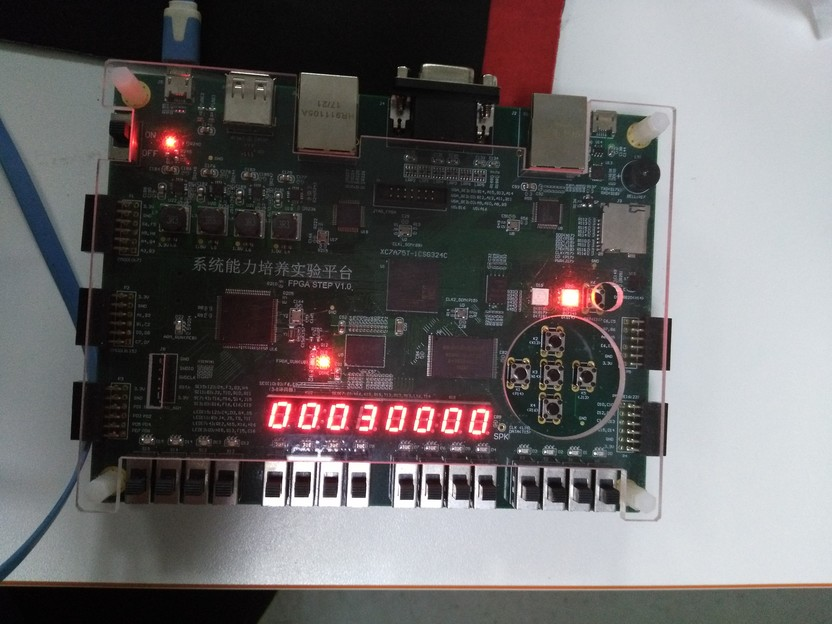
\includegraphics[width=.7\textwidth]{init.jpg}
		\item 通过左右键调节当前歌曲,按下中间按钮,此时左侧红色蓝色LED亮表示开始播放。\footnote{歌曲播放结束后会重新开始播放}

		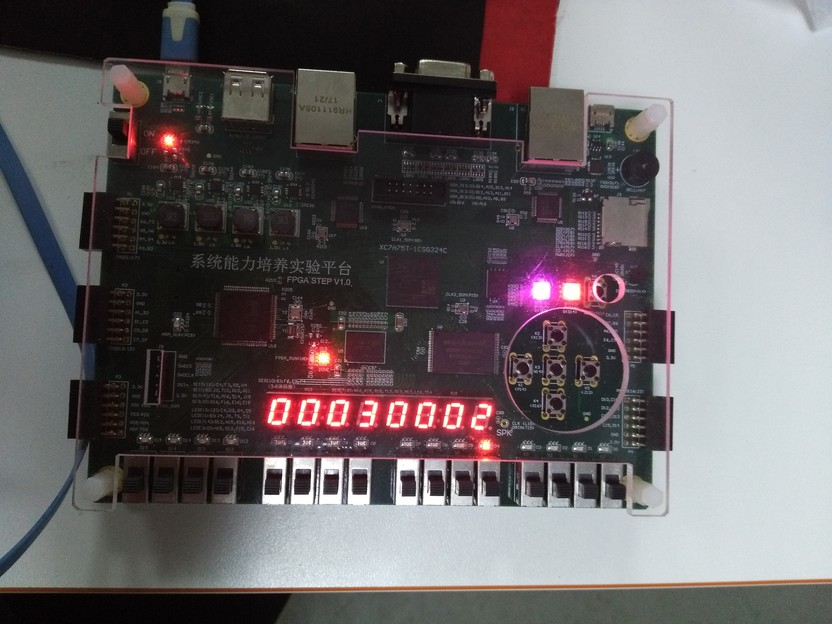
\includegraphics[width=.7\textwidth]{music1.jpg}
		\item 通过上方按钮调节当前模式,当前切换到音乐演奏模式\footnote{播放/暂停状态不会随模式切换改变}。拨动开关会发出相应声音且开关上方LED会亮。\autoref{fig:play}左发出的音为$^\# F_4$,\autoref{fig:play}右发出的音为$^\# A_4$。。

		\begin{figure}[h]
			\caption{演奏模式}
			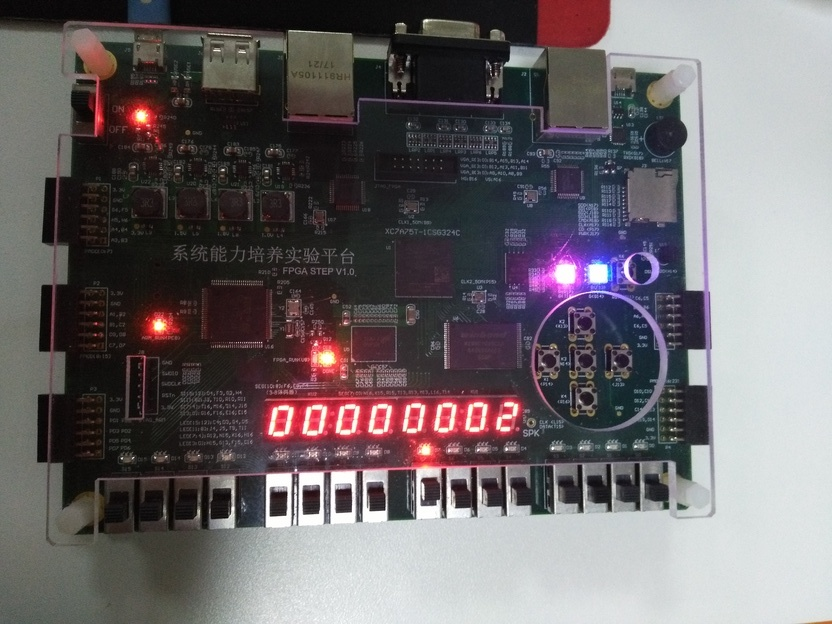
\includegraphics[width=.5\textwidth]{play1.jpg}
			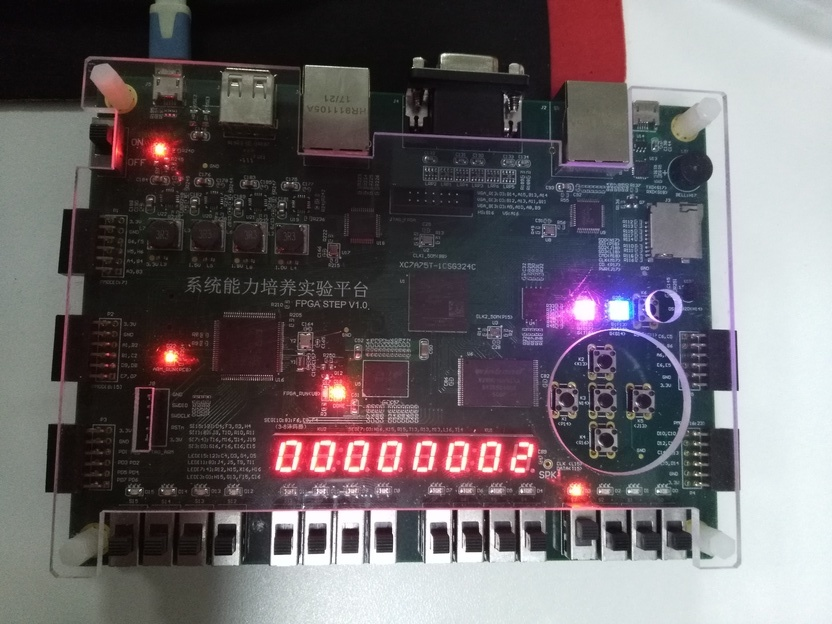
\includegraphics[width=.5\textwidth]{play2.jpg}
			\label{fig:play}
		\end{figure}
		\item 通过左右按钮调节当前音符高低\footnote{播放模式共有8个八度(按照钢琴),但由于蜂鸣器性质,频率段调至5之后的音很难听}。当前音符为$^\# A_{-1}$(由于处于暂停状态,此时不发出声音)。

		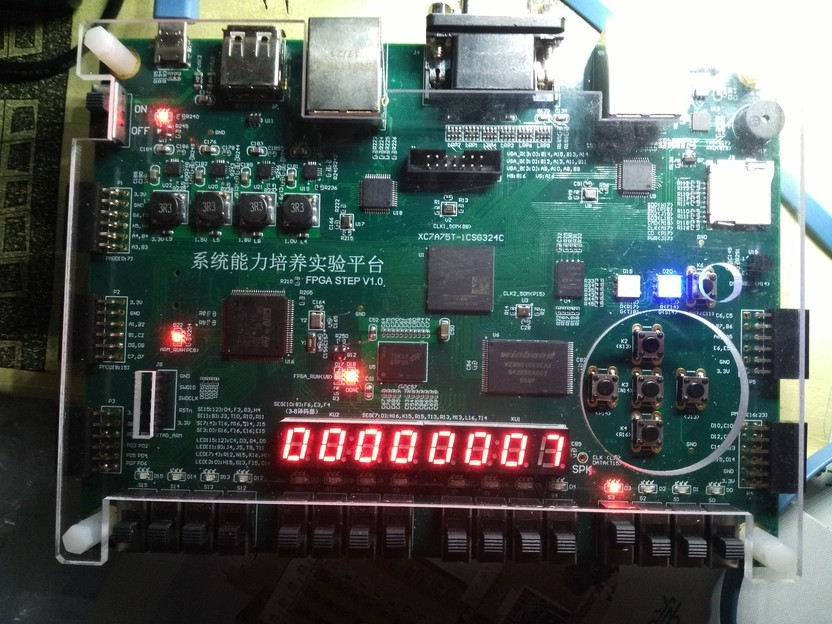
\includegraphics[width=.7\textwidth]{play3.jpg}
		\item 右侧绿灯亮起时,进入写入模式,此时需将另一个usb接口连接电脑,通过python写入数据,数码管左侧显示的为当前写入的地址(寄存器的索引),右侧为当前读入的8bit信息的内容。

		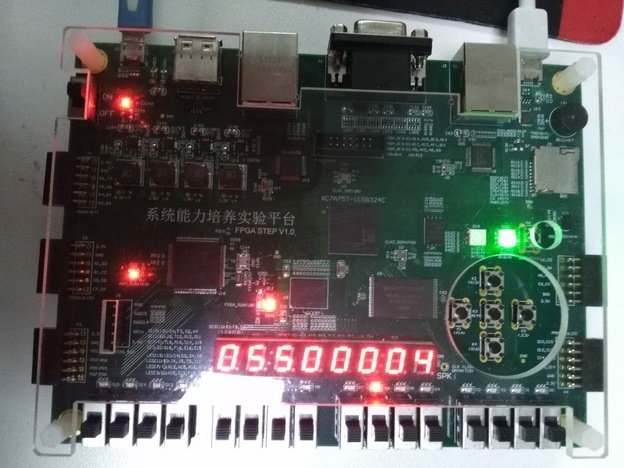
\includegraphics[width=.7\textwidth]{write.jpg}
	\end{enumerate}
	\section{原理}
	\subsection{播放原理}
	本音乐盒以音乐播放模块为基础,以$2093Hz-3951Hz$为基础,设数码管显示的数字为a,则实际频段为$2093 \times 2^a Hz - 3951 \times 2^a Hz$,中间12个开关触发当前频段上的C$-$B音,左侧两个为$a-1$频段的$ .^\# A, B$,右侧两个为$a+1$频段的$C, ^\# C$,寄存器内存储的数据每条长12bit,前四位为音名(与开关作用相同),中间三位为频段(与音乐演奏时数码管上显示的值作用相同),最后五位为时长,以16分音符为单位,时长为该值与16分音符时长的乘积。经过当前音的时长时间再读下一条数据。因此由串口输入的数据也必须按照此格式。
	\subsection{串口通信原理}
	采用的是python的serial库用来写入数据,在没有有效数据传输时,串口始终保持高电平,当准备传输数据时,变为低电平,每位数据保持 1/波特率 时间,8bit数据(1byte)传输之后重新进入高电平状态,等待下一次数据传入。

	因此fpga端的串口接收使用有限状态机,使用时钟信号产生每 $1/2\times$波特率 时间反转一次的脉冲信号作为控制信号。开始处于IDLE状态等待接收,当接收到0之后进入RECV状态,每次控制信号上升沿读一次数据(使用移位寄存器),读完8位之后进入END状态,END状态则输出读出的数据,然后直接跳转到IDLE状态等待下一byte数据。
	\subsection{模块}
	\begin{enumerate}
		\item decode(音乐播放模块,从regfile中提取数据解码得到musicbox模块能读取的数据。
		\item musicbox(主模块,负责发出声音,调节频率段等)
		\item no\_fitter(去抖动模块,负责几个按钮的去抖动)
		\item regfile(寄存器文件,负责存储预置音乐及后面的写入)
		\item seg(数码管解码,负责将由model\_ctl模块输出的32位数据解码成七段数码管可读的数据)
		\item model\_ctl(模块控制,负责根据模式按钮调整模式并相应地改变连线)
		\item uart(串口通信模块,负责从串口中读取数据并将数据解码传递给regfile模块写入)
		\item top(顶层模块,负责模块之间的连线)
	\end{enumerate}
	\subsection{总结}
	\begin{enumerate}
		\item 仍然在变量声明时的长度问题上反了许多错,导致浪费了很多时间。
		\item 敏感变量不能随便使用,其他变量与clk混用时可能会造成竞争。
		\item 对串口通信原理没有理解完全,导致最后write模式仍有些bug。
	\end{enumerate}
		\end{document}
